\documentclass{beamer}
\usepackage{amsfonts,amsmath,oldgerm}

% \usepackage[utf8]{inputenc}
% \usepackage[T1]{fontenc}
\usepackage{graphicx}
\usepackage{listings}
\usepackage{hyperref}
\usepackage{verbatim}
\usepackage{siunitx}
\usepackage{bm}
\usepackage{minted}

\usepackage{color}
\definecolor{bg}{rgb}{0.0,0.95,0.95}

\usepackage{fontspec,unicode-math}
\setmonofont{DejaVuSansMono}[Scale=0.8]



\usepackage[english]{babel}
\usepackage[export]{adjustbox}
\usepackage{caption} %For subfigures
\usepackage{subcaption} %For subfigures
\usepackage{placeins} %FloatBarriers

\usetheme{sintef}

\newcommand{\testcolor}[1]{\colorbox{#1}{\textcolor{#1}{test}}~\texttt{#1}}

\usepackage{biblatex}
\bibliography{bibliography.bib}

\usefonttheme[onlymath]{serif}
\graphicspath{{assets/images/}}


\titlebackground*{assets/logos/background}


\newcommand{\hrefcol}[2]{\textcolor{cyan}{\href{#1}{#2}}}

\title{Numerical study of the airflow over a high-altitude pseudo-satellite wing}
\subtitle{Adjoint Implementation}

\author{\href{mailto:mail@carlobrunelli.com}{Carlo Brunelli}}


\newcommand{\VV}[1] {\vv{\vv{#1}}}

\begin{document}
\maketitle


\section{Implementation}
\begin{frame}{Continuous Adjoint}
\begin{itemize}
\item Continuous Adjoint: equations available
\item Steady (an unsteady version is also implemented, is just faster for validation)
\item Stabilized: SUPG stabilization - same order element interpolation
\end{itemize}
\end{frame}


\begin{frame}[fragile]{Procedure}
Define the objective function $I$ to minimize (eg: Drag coefficient)

\begin{minted}{julia1}
function compute_drag(uh,ph,nΓ,dΓ,params)
    CD, _ = compute_airfoil_coefficients(uh,ph,nΓ,dΓ,params)
    return CD, CD
end
\end{minted}

\begin{minted}{julia1}
function compute_airfoil_forces(uh,ph,nΓ,dΓ,params::Dict{Symbol,Any})
    @unpack tagname,ν = params
    IForce = ∫(-ph ⋅ nΓ + ν* transpose(∇(uh)) ⋅ nΓ)dΓ
    D,L = sum(IForce)
    return D,L
end
\end{minted}
\end{frame}


\begin{frame}[fragile]{Procedure}
Solve the primal Flow
  \begin{minted}[fontsize=\footnotesize]{julia1}
function primal_steady_SUPG(params::Dict{Symbol,Any})
@unpack ν, dt, dΩ, D, Ω, θ,uh = params
h = h_param(Ω, D)
updatekey(params, :h,h)
a((u, p), (v, q)) = ∫(ν * ∇(v) ⊙ ∇(u) + ∇(p) ⊙ v + q * (∇ ⋅ u))dΩ + ∫(v ⊙ (conv ∘ (uh, ∇(u))))dΩ
Rm(u, p) = conv ∘ (uh, ∇(u)) + ∇(p)
astab((u, p), (v, q)) = ∫( τsu(uh, h,ν,dt) ⋅ (uh ⋅ ∇(v) + ∇(q)) ⊙ Rm(u, p))dΩ 
+ ∫( τb(uh, h,ν,dt) ⋅ (∇ ⋅ v) ⊙ (∇ ⋅ u))dΩ
res_prim((u, p), (v, q)) = a((u, p), (v, q)) + astab((u, p), (v, q))
return res_prim
end
\end{minted}
\end{frame}


\begin{frame}[fragile]{Procedure}
  Solve the adjoint Flow
    \begin{minted}[fontsize=\footnotesize,bgcolor=bg]{julia1}
  function adjoint_steady_SUPG(params::Dict{Symbol,Any})
    @unpack ν, dt, dΩ, D, Ω, θ,uh = params
    h = h_param(Ω, D)
    updatekey(params,:h,h)   
    Rmadj(u, p) = -uh ⋅ ∇(u) - ∇(u) ⋅ uh - ∇(p)
    Rcadj(u) = -1 .* (∇ ⋅ (u))
    a_adj((u, p), (v, q)) = ∫(ν * ∇(v) ⊙ ∇(u) - q * (∇ ⋅ u))dΩ + ∫(v ⊙ Rmadj(u, p))dΩ
    a_adj_stab((u, p), (v, q)) = ∫( τsu(uh, h,ν,dt) ⋅ (-uh ⋅ ∇(v) - ∇(v) ⋅ uh - ∇(q)) 
                  ⊙ Rmadj(u, p))dΩ + -1 * ∫( τb(uh, h,ν,dt) ⋅ (∇ ⋅ v) ⊙ Rcadj(u))dΩ
    res_adj((u, p), (v, q)) = a_adj((u, p), (v, q)) + a_adj_stab((u, p), (v, q))
    return res_adj

end
  \end{minted}
  \end{frame}

\begin{frame}[fragile]{Parametrization}
    The airfoil is parametrized using Class Shape Transformations (CST), to obtain easily arifoil-like shapes.
    We start from from a classic NACA0012 airfoil.
    Identified by CST weights for top and bottom surface:
    \begin{minted}[fontsize=\footnotesize,bgcolor=bg]{julia1}
      wu = [0.17085744048372403, 0.15451770272052714, 0.15810479767059346, 0.1359573306370066,
       0.14221259398479932, 0.14001089993692417]
      wl = -1 .* [0.17085744048372403, 0.15451770272052714, 0.15810479767059346, 0.1359573306370066, 
      0.14221259398479932, 0.14001089993692417]
    \end{minted}
    6 parameters for the top, and 6 for the bottom surface: $\beta_i$, $i=1,...,12$, $i=1,...6$: top, $i=7,...12$ bottom.
    
\end{frame}

\begin{frame}[fragile]{Computing Reference values}
Both primal and adjoint flow are solved on the original mesh $\Omega$.
$$I = I_c + \int_\Omega\Psi\cdot\mathcal{R} = I_{1,ref}+I_{2,ref} $$

If we want to minimize $C_D$: $I_c=C_D$
\begin{minted}[fontsize=\footnotesize,bgcolor=bg]{julia1}
  I2 = sum(∫(ϕu⋅((∇(uh))'⋅uh + ∇(ph)))dΩ + ∫(ϕp⋅(∇⋅(uh)))dΩ)
\end{minted}
\end{frame}


\begin{frame}{Morphing mesh}
  \begin{enumerate}
    \item A design variable $\beta_i$ is perturbed by $\epsilon$:  $\beta_i+\epsilon$ 
    \item The airfoil boundary and the mesh move accordingly obtaining a new $\Omega'$ domain
    \item Evaluate $$I' = I_c' + \int_{\Omega'}\Psi\cdot\mathcal{R} = I_{1,i}+I_{2,i} $$
    \item The sensitivity is obtained through
      $$ \dfrac{\partial I }{\partial \beta _ i} = \dfrac{I'-I}{\epsilon}$$
\end{enumerate}

\end{frame}



\begin{frame}{Morphing mesh}
  \begin{figure}[h]
     \includegraphics[width=\textwidth]{MeshMorphedAirfoil.png}
    \caption{$\Omega$ in light blue, morphed mesh $\Omega'$ in black. Shift is emphasized for demonstration.}
    \end{figure} 
\end{frame}



\section{Test Cases}
\begin{frame}{Is the Adjoint Flow Solved Correctly?}
Not many quantitative solutions of the adjoint field are available.
From \footfullcite{Sorgiovanni2016} 2 adjoint flows are reported.    
\end{frame}


\begin{frame}{Cylinder Reynolds 50}
    \begin{figure}[h]
        \centering          
        \begin{subfigure}[h]{0.45\textwidth}
                 \centering
            \includegraphics[width=\textwidth]{PaperRef/Cylinder_Uadjoint.png}
       \end{subfigure}
       \hfill	
       \begin{subfigure}[h]{0.45\textwidth}
                \centering
           \includegraphics[width=\textwidth]{MyRes/Cylinder_Uadjoint.png}
        \end{subfigure}
        \caption{Adjoint Velocity}
        \end{figure} 
    \end{frame}
    
    \begin{frame}{Cylinder Reynolds 50}
    \begin{figure}[h]
        \centering          
        \begin{subfigure}[h]{0.45\textwidth}
                 \centering
            \includegraphics[width=\textwidth]{PaperRef/Cylinder_Padjoint.png}
       \end{subfigure}
       \hfill	
       \begin{subfigure}[h]{0.45\textwidth}
                \centering
           \includegraphics[width=\textwidth]{MyRes/Cylinder_Padjoint.png}
        \end{subfigure}
        \caption{Adjoint Pressure}
        \end{figure} 
    \end{frame}

\begin{frame}{NACA0012 $AoA=\ang{2.5}$, $Re=1000$}
Drag minimization.
Boundary conditions:
\begin{itemize}
    \item $\Gamma_{airfoil}: \Psi_u = [-1.0, 0.0]$
    \item $\Gamma_{inlet}:\Psi_p = 0.0$
    \item $\Gamma_{outlet}: \Psi_u = [0.0, 0.0]$
    \item $\Gamma_{limits}: \Psi_u = [0.0, 0.0]$

\end{itemize}
        
\end{frame}

\begin{frame}{NACA0012 $AoA=\ang{2.5}$, $Re=1000$}
\begin{figure}[h]
    \centering          
    \begin{subfigure}[h]{0.45\textwidth}
             \centering
        \includegraphics[width=\textwidth]{PaperRef/NACA0012_Uprimal.png}
   \end{subfigure}
   \hfill	
   \begin{subfigure}[h]{0.45\textwidth}
            \centering
       \includegraphics[width=\textwidth]{MyRes/NACA0012_Uprimal.png}
    \end{subfigure}
    \caption{Primal Velocity}
    \end{figure} 
\end{frame}

\begin{frame}
\begin{figure}[h]
    \centering          
    \begin{subfigure}[h]{0.45\textwidth}
             \centering
        \includegraphics[width=\textwidth]{PaperRef/NACA0012_Pprimal.png}
   \end{subfigure}
   \hfill	
   \begin{subfigure}[h]{0.45\textwidth}
            \centering
       \includegraphics[width=\textwidth]{MyRes/NACA0012_Pprimal.png}
    \end{subfigure}
    \caption{Primal Pressure}
    \end{figure} 
\end{frame}

\begin{frame}
\begin{figure}[h]
    \centering          
    \begin{subfigure}[h]{0.45\textwidth}
             \centering
        \includegraphics[width=\textwidth]{PaperRef/NACA0012_Uadjoint.png}
   \end{subfigure}
   \hfill	
   \begin{subfigure}[h]{0.45\textwidth}
            \centering
       \includegraphics[width=\textwidth]{MyRes/NACA0012_Uadjoint.png}
    \end{subfigure}
    \caption{Adjoint Velocity}
    \end{figure} 
\end{frame}

\begin{frame}
\begin{figure}[h]
    \centering          
    \begin{subfigure}[h]{0.45\textwidth}
             \centering
        \includegraphics[width=\textwidth]{PaperRef/NACA0012_Padjoint.png}
   \end{subfigure}
   \hfill	
   \begin{subfigure}[h]{0.45\textwidth}
            \centering
       \includegraphics[width=\textwidth]{MyRes/NACA0012_Padjoint.png}
    \end{subfigure}
    \caption{Adjoint Pressure}
    \end{figure} 
\end{frame}


\begin{frame}{Finite Difference Tests}
Computing the gradients for a STEADY case. NACA0012, $AoA=\ang{0.0}$, Re=100. 
In FD, each $\beta_i$ is perturbed by $\epsilon$ and the flow is solved. 
$$ \dfrac{\partial C_D }{\partial \beta _ i} = \dfrac{C_D'-C_D}{\epsilon}$$

Gradients computed with FD and Adjoind should be the same, but they are not. The perturbation $\epsilon$ is the same for FD and adjoint.
\begin{figure}[h]
    \centering          
        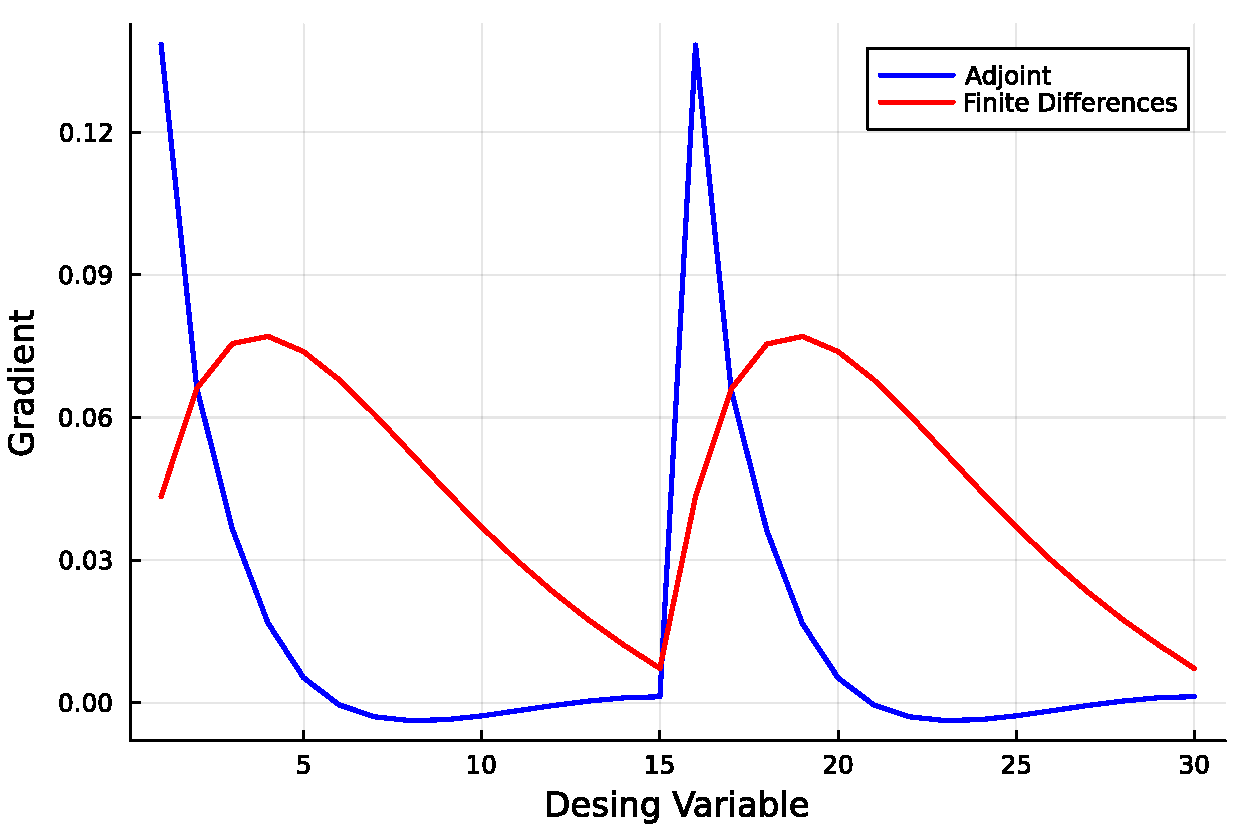
\includegraphics[width=0.3\textwidth]{Adjoint_FD.pdf}
       \caption{$C_D$ gradient, finite difference vs adjoint}
    \end{figure} 
\end{frame}

\begin{frame}{Finite Difference Tests}
Gradients are symmetric in top and bottom design variables
Order of magnitude really are close but not matching 
\end{frame}

\section{Considerations}
\begin{frame}
    \begin{itemize}
        \item Gradients for FD and Adjoint do not depend on $\epsilon$. $\epsilon=0.001$, same results for $\epsilon=0.01,0.0001$.
        \item FD and Adjoint different results, but at least the sign is the same
        \item The adjoint results are sensible to the boundary condition on the airfoil surface. Fixing $\Psi_u = [-1.0, 0.0]$ or $\Psi_u = [-C_D, 0.0]$ impact the gradients.
        \item Error in boundary conditions? The error should be eliminated due to the difference $I'-I$.
    \end{itemize}
\end{frame}

\end{document}
